\documentclass[12pt,a4paper]{article}
\usepackage[utf8]{inputenc}
\usepackage[T1]{fontenc}
\usepackage{amsmath}
\usepackage{textcomp}

\usepackage{geometry}
\geometry{a4paper,left=25mm,right=25mm, top=2cm, bottom=2cm} 

\usepackage{graphicx} %fuer bilder

\usepackage{verbatim}


\usepackage{pgfplots}

 \usepackage{mathptmx}
 \usepackage[scaled=.90]{helvet}
 \usepackage{courier}



\usepackage{listings}
\usepackage{color}

\usepackage{float}
 
\definecolor{dkgreen}{rgb}{0,0.6,0}
\definecolor{gray}{rgb}{0.5,0.5,0.5}
\definecolor{mauve}{rgb}{0.58,0,0.82}

\pagestyle{empty}
\lstset{numbers=left,language=C++}
\lstset{showstringspaces=false,
basicstyle=\ttfamily\footnotesize,
breaklines=true,
tabsize=3,
commentstyle=\color{dkgreen},      % comment style
inputencoding={ansinew},
title=\lstname %zeigt titel der datei an
}

\usepackage{pdfpages} % fuer pdfs
\usepackage{hyperref} % fuer url

%keine einrückungen bei absatz
\parindent 0pt

\begin{document}
\title{Übung 10}
\author{Reinhard Penn, Bernhard Selymes}
\date{Juni 2015}

\normalsize

%Beginn des Dokuments

\newcommand{\srcpath}{../../src}
\newcommand{\simpath}{../../sim}

%Angabe
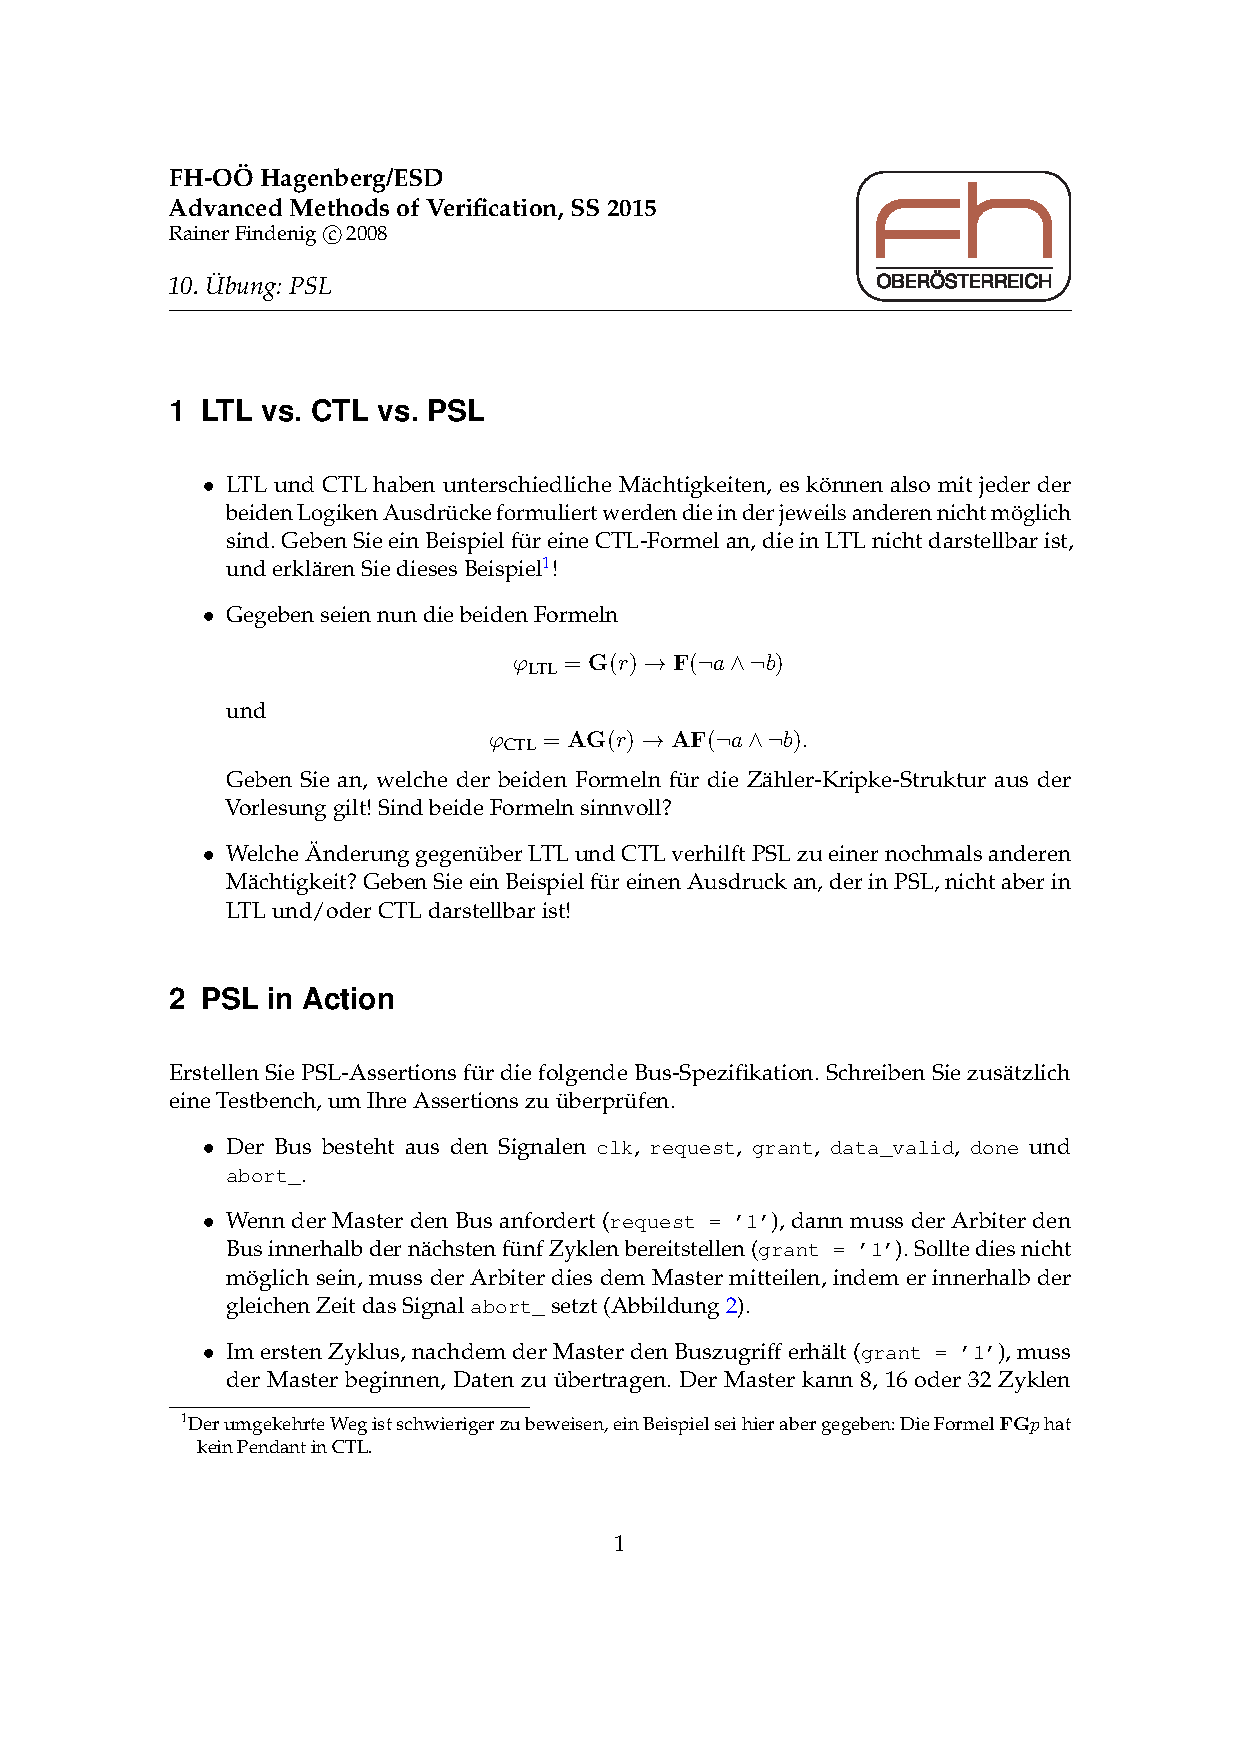
\includepdf[pages=-]{../Angabe.pdf}

\section{LTL vs. CTL vs. PSL}

\begin{itemize}
	\item Die Formel 
		\begin{equation*}
			\varphi_{CTL} = \textbf{EG}\textit{p}
		\end{equation*}
		ist nur in CTL möglich, da sie eine Aussage über die Existenz eines Pfades ist, was in LTL nicht möglich ist.
	\item Die LTL-Formel entspricht dem Reset und gilt für die Zähler-Kripke-Struktur aus der Vorlesung. Die CTL-Formel gilt nicht und ist sinnlos.
	\item Die Erweiterung mit regulären Ausdrücken verhilft PSL zu einer höheren Mächtigkeit.
				\begin{verbatim}
				assert always (a -> {next_a}[3:5](b));
				\end{verbatim}
				Wie man in diesem Beispiel sieht kann die PSL auch zählen, was in CTL und LTL nicht möglich ist.
\end{itemize}

\section{PSL in Action}


\lstinputlisting[language={vhdl}]{\srcpath/SimpleBus-Bhv-ea.vhd}
\lstinputlisting[language={verilog}]{\srcpath/vunit.psl}
\lstinputlisting[language={tcl}]{\simpath/ComSim.do}

\end{document}
